\section{Likelihood Method}

In this section timing cuts for discriminating between pion, kaon, and proton tracks are described.  Each positive track is assigned an identity based on the largest likelihood ratio of the three candidates.  There may be times when although a track is categorized as one particle species, it is very unlikely (all likelihood values were small). The analyst can use a consistency test to discard such events.  The calculation of significance levels for this purpose will also be discussed.  \\

\subsection{Likelihood Functions}

For each particle species considered, a normalized probability density function $P(x;p,h)$ is constructed for each input into the likelihood analysis.  Here, x corresponds to the feature being used to catagorize different particles (x could be delta-beta, time of flight, or energy deposition etc.), p is the particle momentum, and h is the hadron being hypothesized (eg: in our case the possible values for h are pion, kaon, proton).  If one uses a set of $N$ variables $x = (x_1, x_2, ..., x_N)$, the likelihood for a hypothesis h can be defined as shown below. 

\begin{equation}
  \mathcal{L}_h = \prod_{N}^{i=1} P_{i} (x_i; p, h)
\end{equation}

In many cases, it is possible to use a Gaussian PDF for the variable $x_i$, and fixed values of p, h.

\begin{equation}
  P(x_i;p,h) = \frac{1}{\sqrt{2 \pi} \sigma_i(p,h) } exp \left \{ -\frac{1}{2} \bigg( \frac{x_i - \mu_i(p,h)}{\sigma_i(p,h)} \bigg)^2 \right \}
\end{equation}

The identity is assigned by choosing the particle hypothesis h which maximizes the likelihood ratio.  Using this method, every positive track is assigned a particle identification.  However, at times the likelihood value is quite small when compared with the maximum likelihood for that species.  This is the case for positrons which are classified by this method as positive pions, because they are the closest particle for which a hypothesis has been provided.  To avoid these situations, the significance level of each track is calculated and a cut is placed on the minumum significance.  The effect of this cut on the analysis can be easily measured as significance level is bound between 0 and 1.  

\begin{equation}
  S = 1 - \int_{\mu-x_{obs}}^{\mu-x_{obs}} P(x_i;p,h) dx_i 
\end{equation}

This quantity represents the probability to observe a value of x as far from the mean as $x_{obs}$.  Significance levels of 0 then correspond to tracks which are poorly identified as the class h.  In the case that the PDF is Gaussian, the standard 1, 2, and 3 sigma cuts can be understood simply as significance levels of approximately 0.32 = 1-0.68, 0.05 = 1-0.95, and 0.01 = 1-0.99.

\begin{equation}
  \frac{\mathcal{L}_h}{\mathcal{L}_{\pi^+}+\mathcal{L}_{K^+}+\mathcal{L}_{p}}
\end{equation}

\begin{figure}
  \begin{center}
    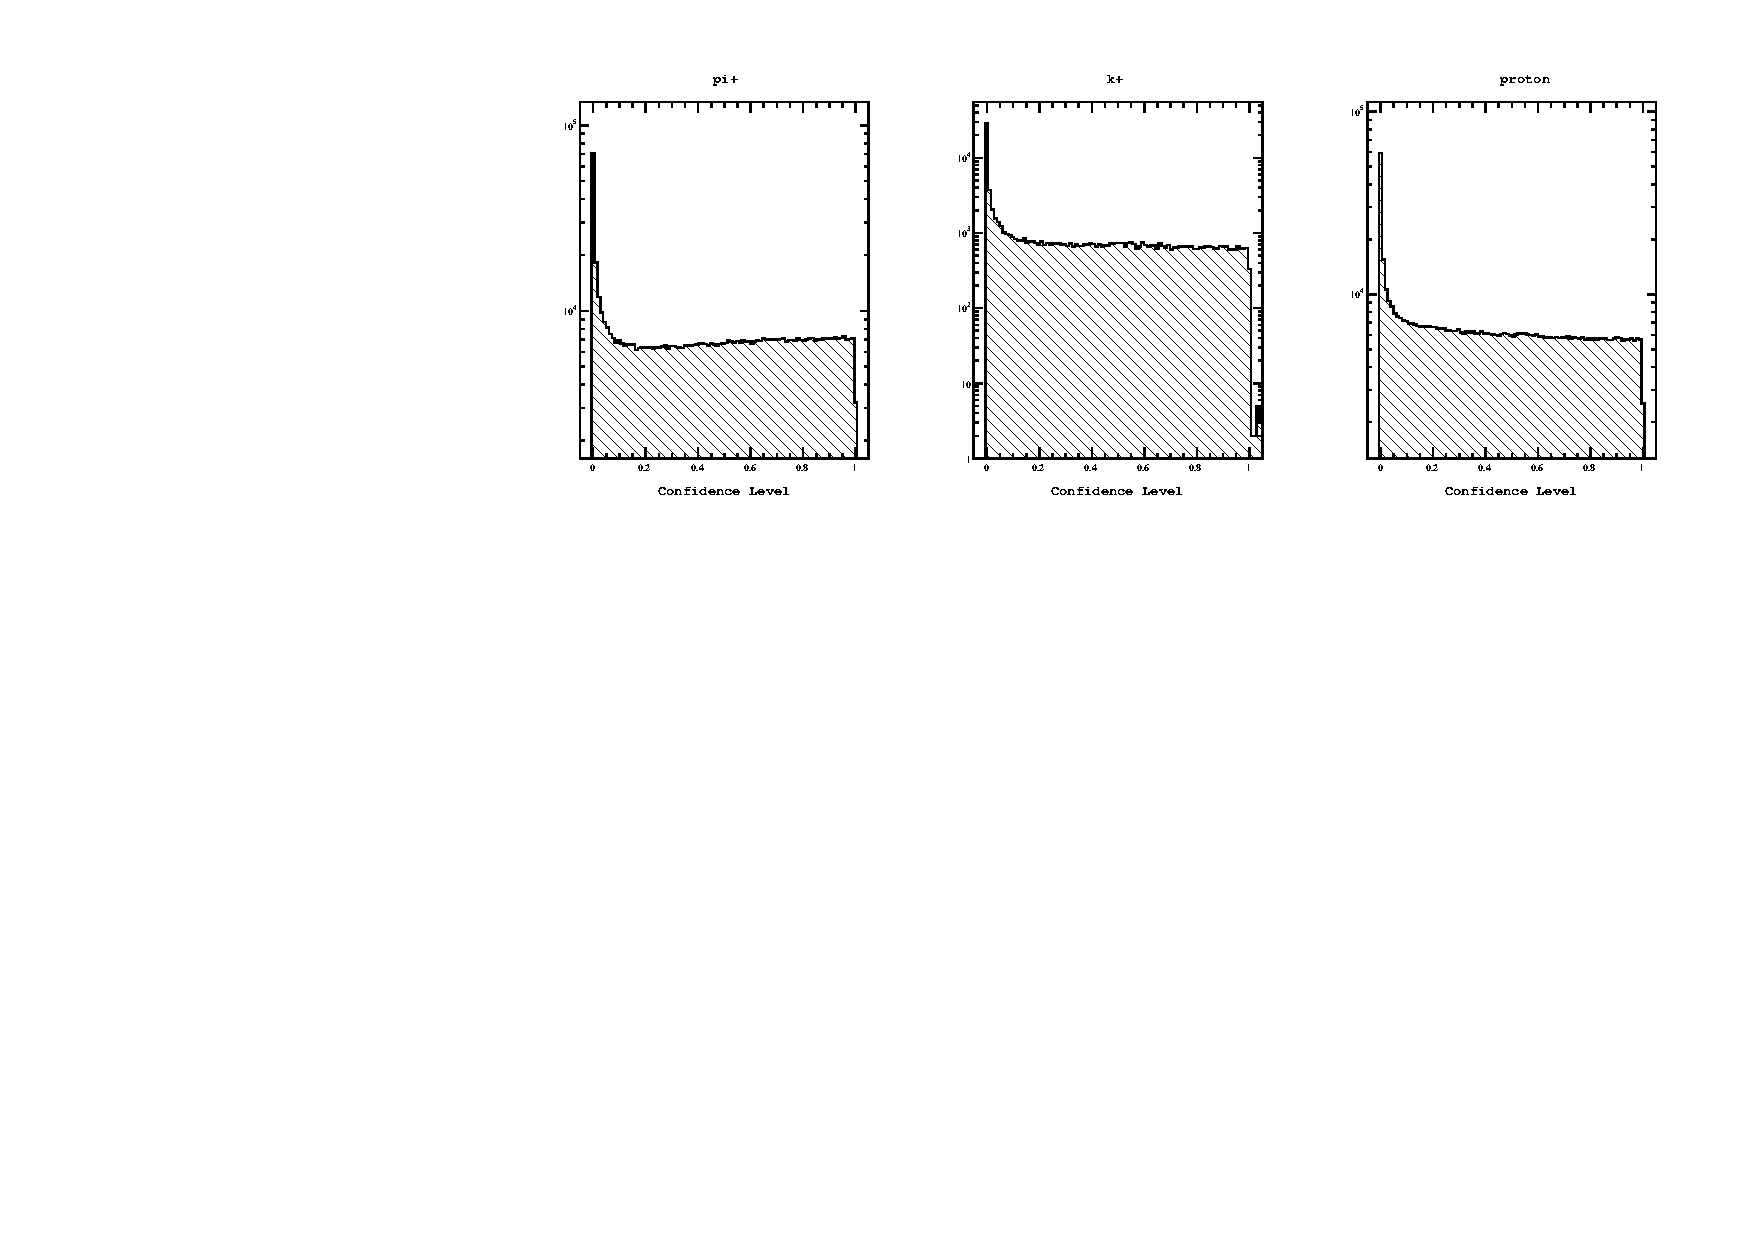
\includegraphics[width=10cm]{image/confidence_level.pdf}
    \caption{ Shown above: }
  \end{center}
\end{figure}

\begin{figure}
  \begin{center}
    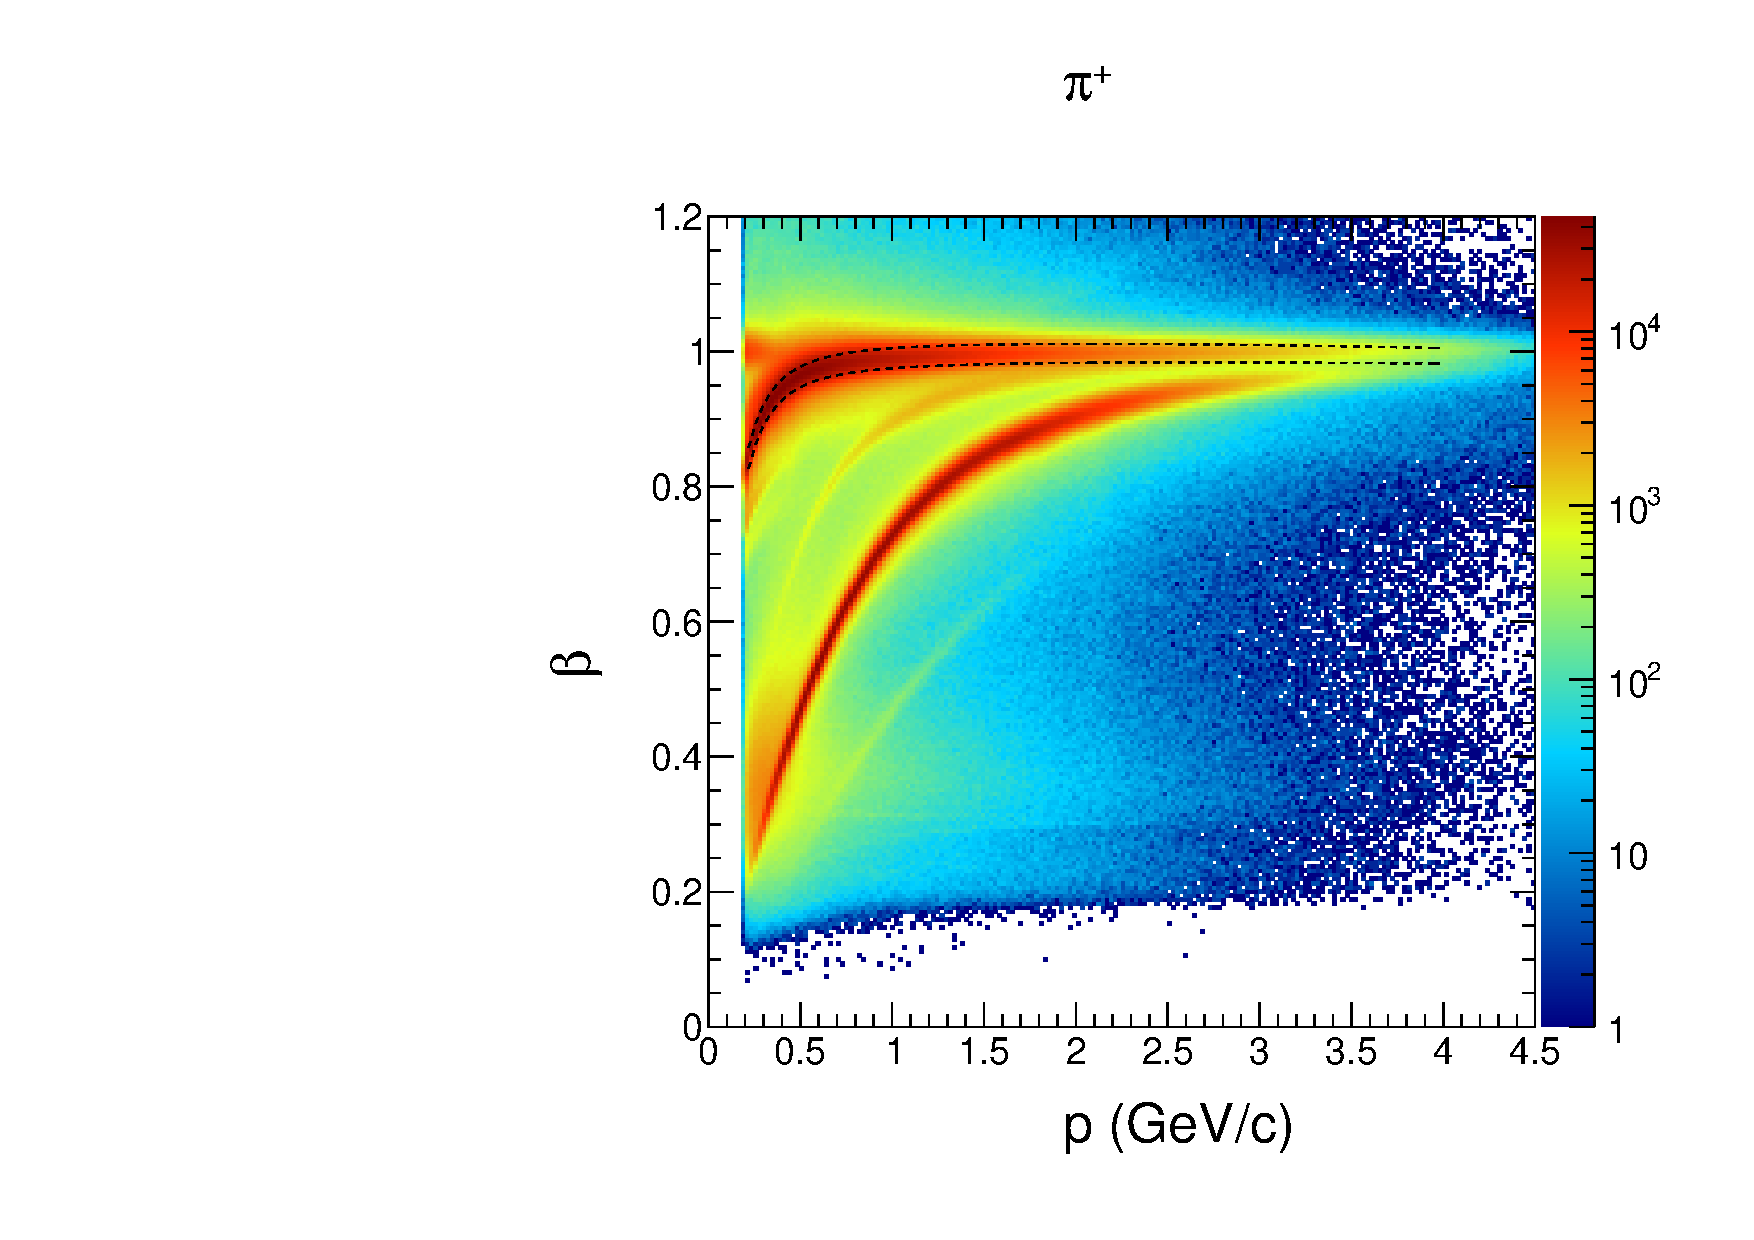
\includegraphics[width=10cm]{image/beautiful_pbeta_pip.pdf}
    \caption{ Shown above: }
  \end{center}
\end{figure}

\begin{figure}
  \begin{center}
    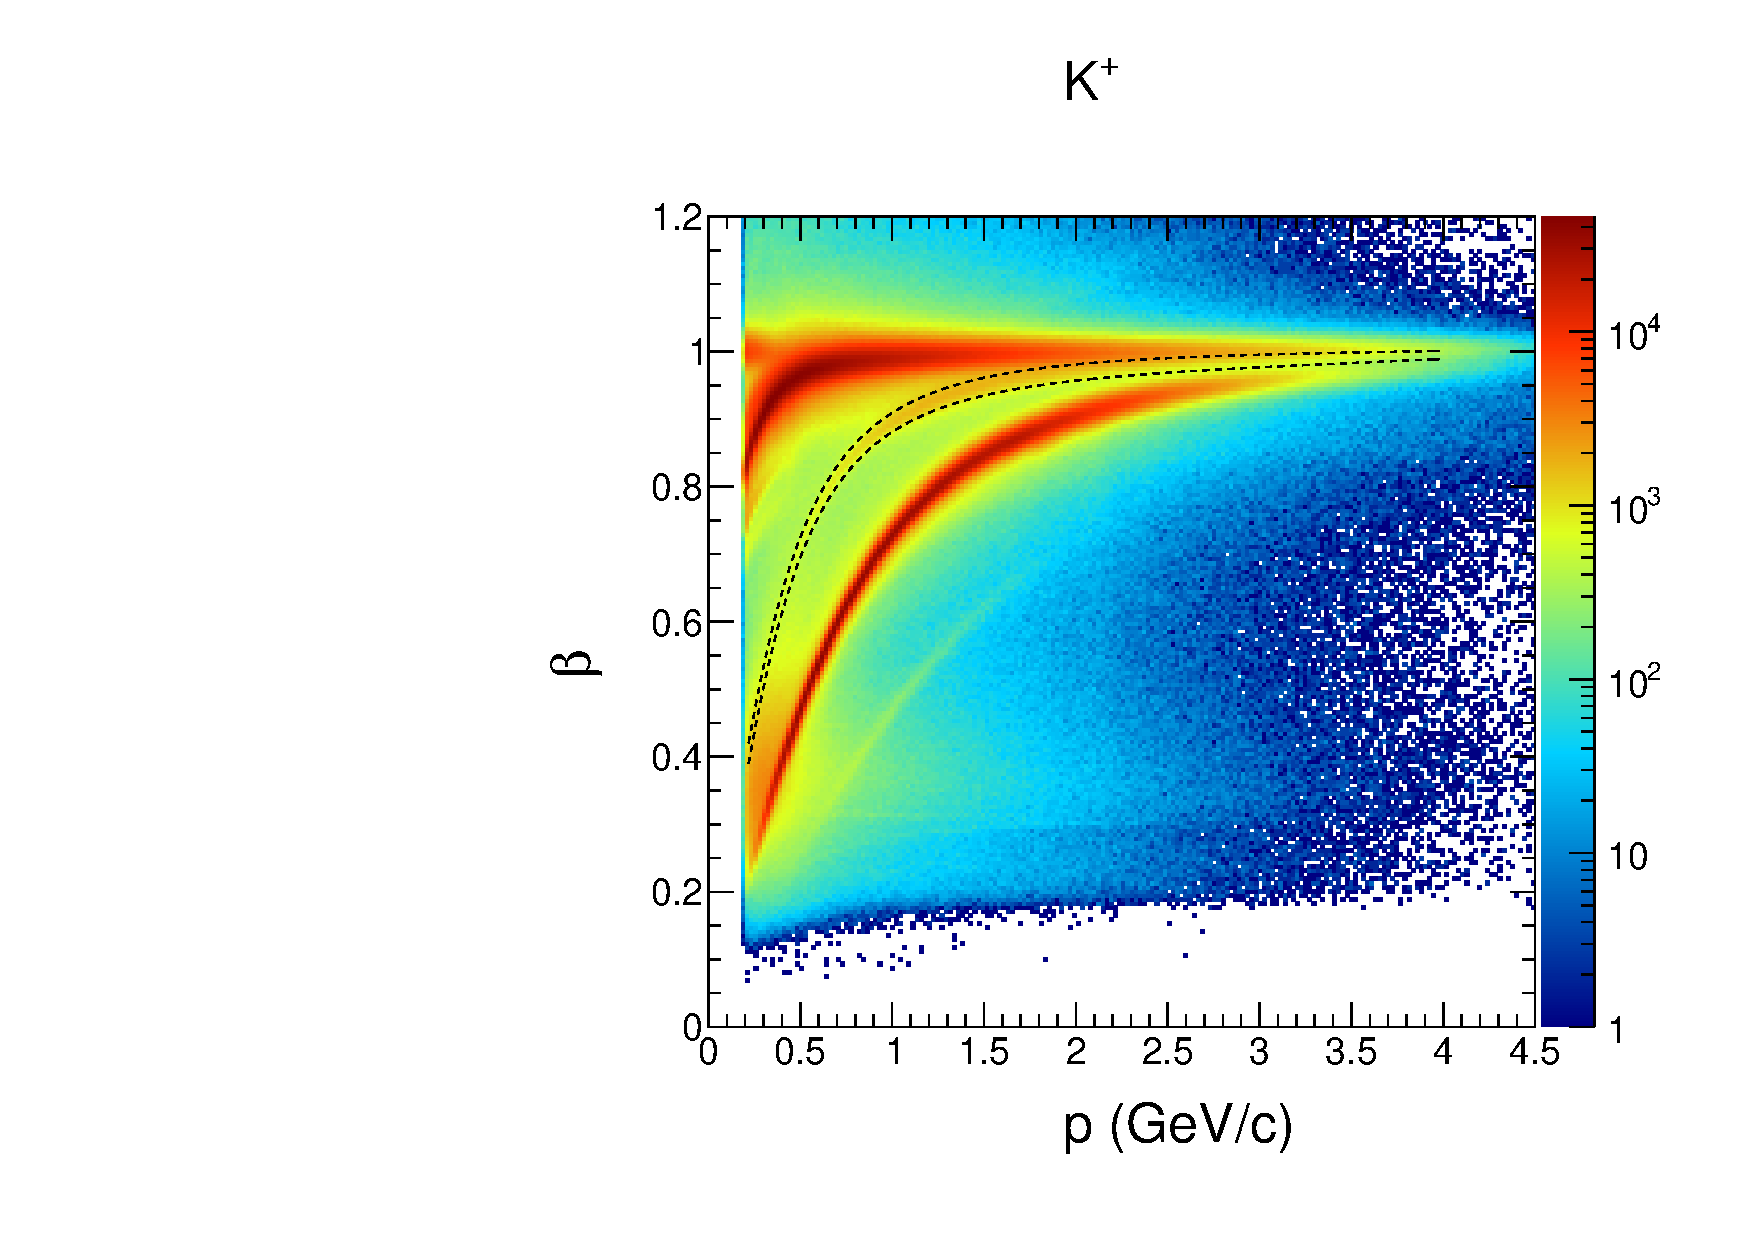
\includegraphics[width=10cm]{image/beautiful_pbeta_kp.pdf}
    \caption{ Shown above: }
  \end{center}
\end{figure}

\begin{figure}
  \begin{center}
    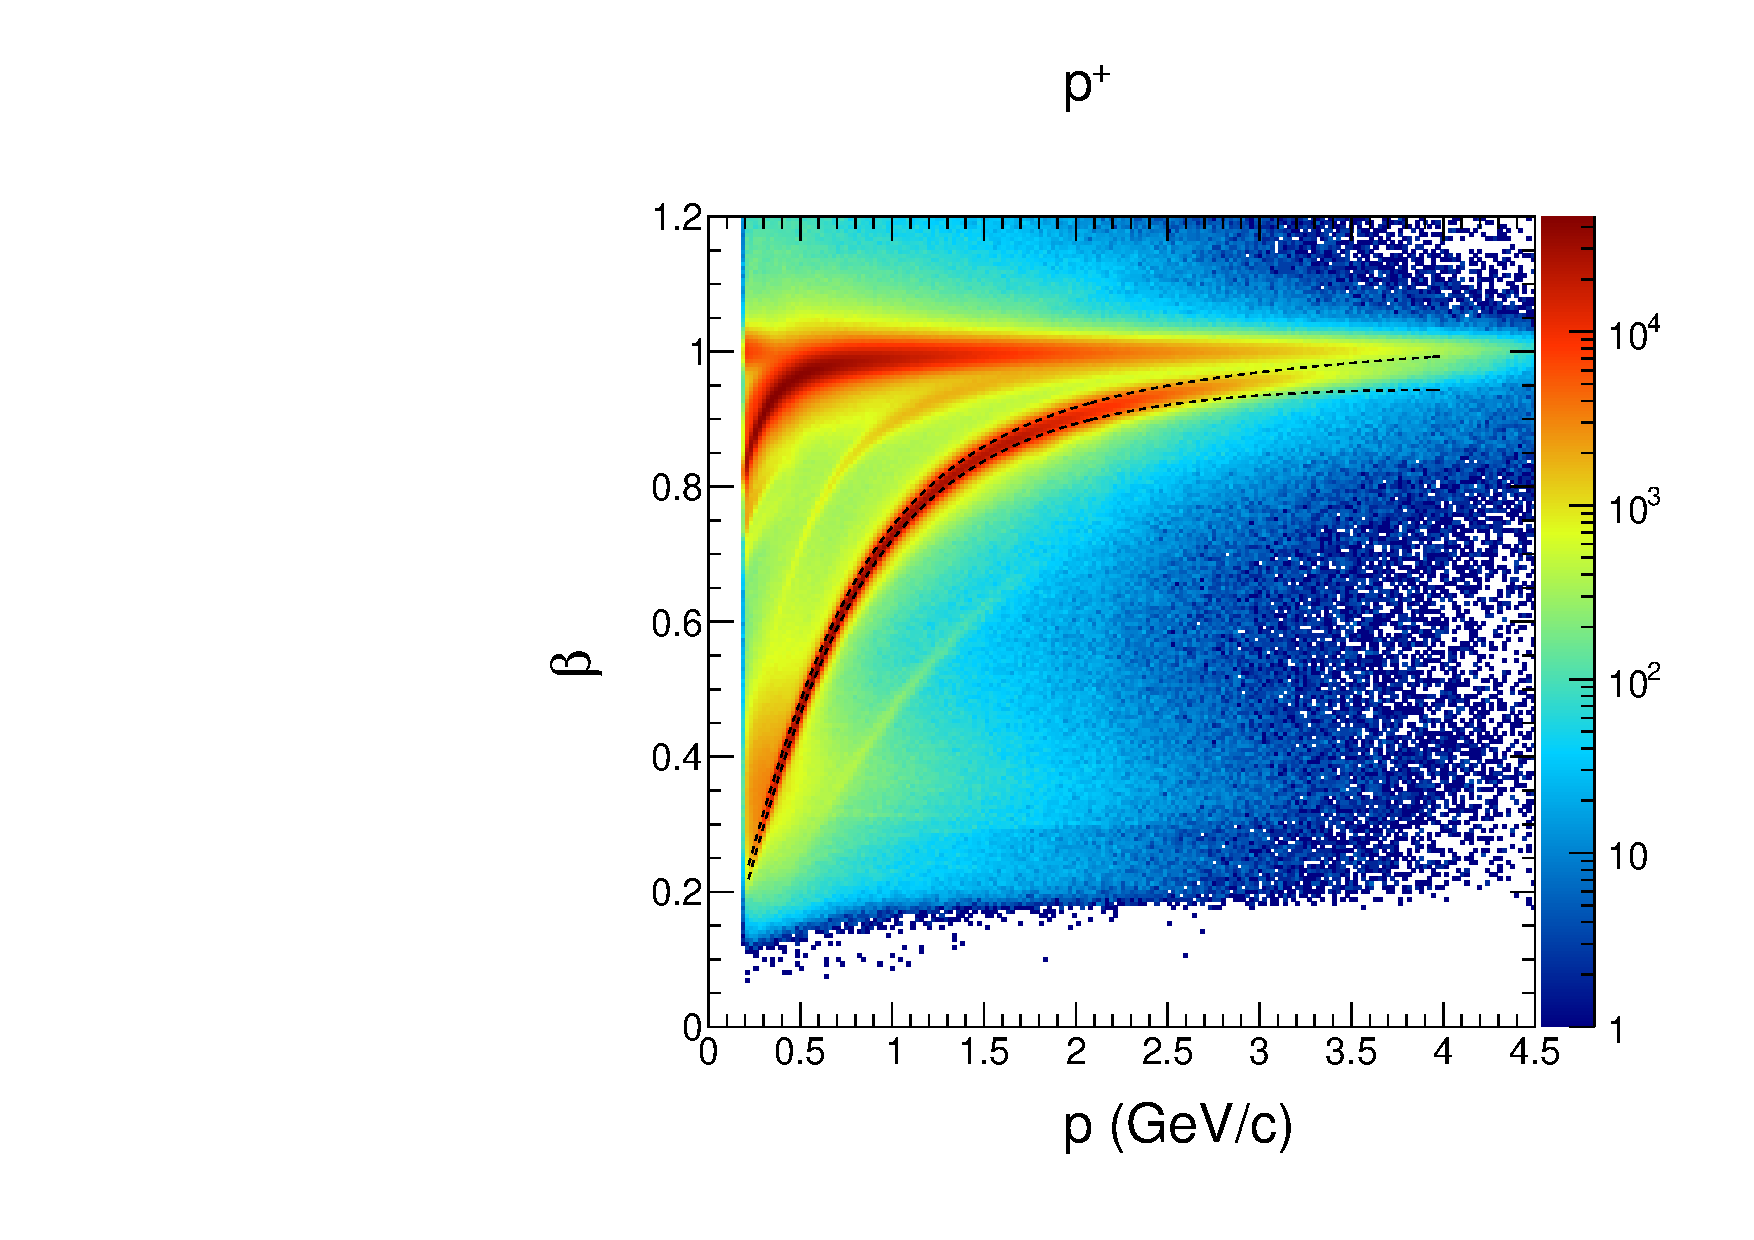
\includegraphics[width=10cm]{image/beautiful_pbeta_prot.pdf}
    \caption{ Shown above: }
  \end{center}
\end{figure}

\begin{itemize}
  \item theory 
  \item resolution fits 
  \item confidence level plots
\end{itemize}



